\documentclass[a4paper,11pt]{article} 
\usepackage[T1]{fontenc} 
\usepackage{times} 
\usepackage{mathtools}
\usepackage[swedish,english]{babel} 
\usepackage[utf8]{inputenc} 
\usepackage{dtk-logos} 
\usepackage{wallpaper} 
\usepackage[absolute]{textpos} 
\usepackage[top=2cm, bottom=2.5cm, left=3cm, right=3cm]{geometry} 
\usepackage[parfill]{parskip} 
\usepackage{csquotes} 
\usepackage{float} 
\usepackage{lipsum}
\usepackage{graphicx}
\usepackage[nottoc]{tocbibind} % BibTex References
\usepackage{sectsty} % No section number 

\usepackage{sectsty} 
\sectionfont{\fontsize{14}{15}\selectfont}
\subsectionfont{\fontsize{12}{15}\selectfont}
\subsubsectionfont{\fontsize{12}{15}\selectfont}

\newsavebox{\mybox}
\newlength{\mydepth}
\newlength{\myheight}

\setlength{\parindent}{1cm} %Added for paragraph indentation 
\newenvironment{sidebar}%
{\begin{lrbox}{\mybox}\begin{minipage}{\textwidth}}%
{\end{minipage}\end{lrbox}%
 \settodepth{\mydepth}{\usebox{\mybox}}%
 \settoheight{\myheight}{\usebox{\mybox}}%
 \addtolength{\myheight}{\mydepth}%
 \noindent\makebox[0pt]{\hspace{-20pt}\rule[-\mydepth]{1pt}{\myheight}}%
 \usebox{\mybox}}

\newcommand\BackgroundPic{
    \put(-2,-3){
    
\includegraphics[keepaspectratio,scale=0.3]{lnu_etch.png}
    }
}
\newcommand\BackgroundPicLogo{
    \put(30,740){
    
\includegraphics[keepaspectratio,scale=0.10]{logo.png} 
    }
}

\title{
\vspace{-8cm}
\begin{sidebar}
    \vspace{10cm}
    \normalfont \normalsize
    \huge Operating Systems\\ 
    \vspace{-1.3cm}
\end{sidebar}
\vspace{3cm}
\begin{flushleft}
    \huge Chapter 4 \\ \textit{Threads}
\end{flushleft}
\null
\vfill
\begin{textblock}{5}(10,13)
\begin{flushright}
\begin{minipage}{\textwidth}
\begin{flushleft} \large
\emph{Authors:}\\ Student \textsc{1}\\ Student \textsc{2} \\
\emph{Supervisor:} Teacher\\
\emph{Term:} HT19\\
\emph{Course code:} 1DV512\\ 
\end{flushleft}
\end{minipage}
\end{flushright}
\end{textblock}
}

\date{} 
\author{}  

\begin{document}
\pagenumbering{gobble} 
\newgeometry{left=5cm}
\AddToShipoutPicture*{\BackgroundPic} 
\AddToShipoutPicture*{\BackgroundPicLogo} 
\maketitle 
\restoregeometry
\clearpage

\pagenumbering{gobble}
\selectlanguage{English}
\tableofcontents 

\newpage
\pagenumbering{arabic}
%%%%%%%%%%%%%%%%%%%%%%%%%%%%%%%%%%%%%%%%%%%%%%%%%%%%%%%%%%%%%%%%%%
%                            Threads                            %
%%%%%%%%%%%%%%%%%%%%%%%%%%%%%%%%%%%%%%%%%%%%%%%%%%%%%%%%%%%%%%%%%%
\section{Introduction}
The smallest individual components of CPU utilization are threads. Threads consist of a thread ID, program counter, register set \& a stack. With the other threads that belong to the same process, a thread also shares a code section, data section \& other operating-system resources. Like signals \& open files. A process is either single-threaded or multithreaded. Multithreaded processes, unlike single-threaded processes, can perform multiple tasks at a time. Today most operating-systems are multithreaded thereat all the threads have specific tasks that they operate in the kernel. 
Multithreaded programming has the following advantages:
\begin{description}
    \item[Increased responsiveness: ]A program can continue to run even if some part of it is blocked or takes a lot of time to run. Therefore, an interactive application will not have the user wait for an operation to finish before it is responsive again, which is the case for a single-threaded application. 
    \item[Sharing of resources:]The memory is less affected because the resources of a multithreaded process is automatically shared by the threads it consists of. In extension this also makes multithreaded programming more \textbf{economical} than single-threaded programming. 
    \item[Scalability:]A multiprocessor environment makes multithreading even more beneficial. When available, threads can run in parallel on different cores unlike a single-threaded process that are unable to run on more than one.
\end{description}
%%%%%%%%%%%%%%%%%%%%%%%%%%%%%%%%%%%%%%%%%%%%%%%%%%%%%%%%%%%%%%%%%%
%                     MULTICORE PROGRAMMING                      %
%%%%%%%%%%%%%%%%%%%%%%%%%%%%%%%%%%%%%%%%%%%%%%%%%%%%%%%%%%%%%%%%%%
\newpage\section{Multicore Programming}
Multicore or multiprocessor systems are systems where each core is a separate processor in the operating system. Multithreaded programming makes better use of these multicore systems \& improves concurrency. Concurrency in a multicore system means that a separate thread can be assigned to each core whereas the threads run in parallel, while in a single core system only one thread at a time is being executed. However there is a difference between parallelism \& concurrency, parallel systems simultaneously perform more than one task while concurrent systems allows all tasks to make progress. Therefore parallelism is not required to achieve concurrency. Switching quickly between processes in the system is concurrency but provides the illusion that the system runs in parallel.
\newline\indent The potential gain of implementing an additional core can be calculated by Amdahl’s law (Equation \ref{amdahlslaw}) where N is the number of processing cores in a system \& S the portion of the application that has to be performed serially. 

\begin{equation}
\label{amdahlslaw}
    speedup \leq \frac{1}{S+\frac{1-S}{N}}
\end{equation}
%--------------------- PROGRAMMING CHALLENGES ---------------------%
\subsection{Programming challenges}

Making use of multicore system is a challenge for programmers. The five most common difficulties are: 

\begin{description}
    \item [Identifying Tasks:] Finding \& dividing areas in applications into separate, concurrent tasks.  
    \item [Balance:] Making sure that the tasks running in parallel perform equal work of equal value. 
    \item [Data splitting:] Divide the data accessed \& manipulated by the separated tasks to run on different cores.
    \item [Data Dependency:] Finding dependencies between tasks \& adjusting them by making them synchronized.
    \item [Testing \& debugging:] It is much more difficult to test a multicore program since there are many different execution paths possible. 
\end{description}

The design of software in the future may need a whole new approach because of these difficulties. 
%-------------------- TYPES OF PARALLELISM ----------------------%
\subsection{Types of parallelism}
Generally there are two types of parallelism; data parallelism \& task parallelism.

\begin{description}
    \item [Data parallelism:] Data is divided into subsets \& divided across multiple cores. The same operation is performed on the data but on different cores.
    \item [Task parallelism:] Different tasks are distributed across multiple cores. The same data may be operated on at the same time by different threads. 
\end{description}

Most applications use both data \& task parallelism.

%%%%%%%%%%%%%%%%%%%%%%%%%%%%%%%%%%%%%%%%%%%%%%%%%%%%%%%%%%%%%%%%%%
%                     MULTITHREADING MODELS                      %
%%%%%%%%%%%%%%%%%%%%%%%%%%%%%%%%%%%%%%%%%%%%%%%%%%%%%%%%%%%%%%%%%%
\newpage\section{Multithreading Models}
Multithreading models are used to establish the relationship between user threads \& kernel threads. The difference between user threads \& kernel threads are the way they are supported by the operating system.

\begin{description}
    \item[User threads:] Supported above the kernel \& managed without kernel support.
    \item[Kernel threads:] Supported \& managed directly by the operating system.
\end{description}

The three common models for this relationship that will be presented are many-to-one, one-to-one  many-to-many.

%---------------------- MANY-TO-ONE MODEL -----------------------%
\subsection{Many-to-one model}
One kernel thread has many user-level threads mapped to it. Because of its incapacity to make use of multiple processor cores the many-to-one model (Figure \ref{manytoone}) is rather outdated. 
\begin{figure}[ht]
\centering
[1]
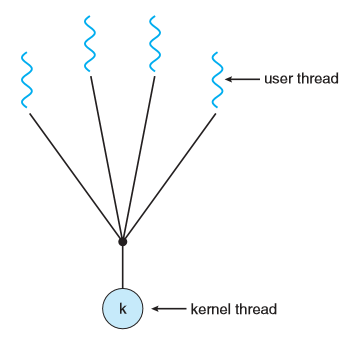
\includegraphics[width=4cm]{1DV512/manyone.png}
\caption{many-to-one}
\label{manytoone}
\end{figure}

\textbf{Disadvantage:} 
\begin{itemize}
    \item If a thread makes a blocking system call the entire process will be blocked.
    \item Multiple threads are unable to run in parallel on multicore system since only one thread at a time can access the kernel. 
\end{itemize}

%----------------------- ONE-TO-ONE MODEL -----------------------%
\subsection{One-to-One Model}
Each user-level thread is distributed to a kernel thread by the one-to-one model (Figure \ref{onetoone}). This allows a thread to run even when another thread is making a blocking system call unlike in the many-to-one model. 

\begin{figure}[ht]
[1]
\centering
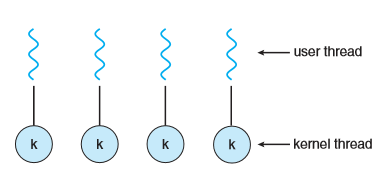
\includegraphics[width=4.5cm]{1DV512/oneone.png}
\caption{one-to-one}
\label{onetoone}
\end{figure}

\textbf{Disadvantage:} 
\begin{itemize}
    \item Implementation will most likely restrict the number of threads supported by the system.
\end{itemize}
%---------------------- MANY-TO-MANY MODEL ----------------------%
\subsection{Many-to-Many Model}
Multiple user-level threads are multiplexed to an equal or smaller number of kernel threads. Therefore the many-to-many model (Figure \ref{manytomany}) manages to avoid the disadvantages of the many-to-one mode \& one-to-one model.

\begin{figure}[ht]
[1]
\centering
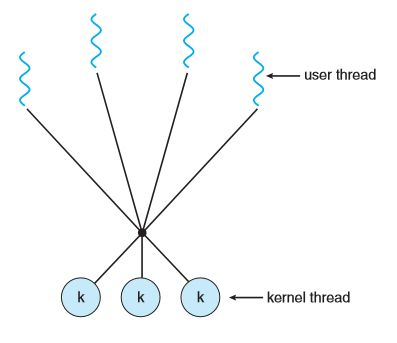
\includegraphics[width=4cm]{1DV512/manymany.png}
\caption{many-to-many}
\label{manytomany}
\end{figure}

Another model that is a variation of the many-to-many model is the two-level model. In addition to having many user-level threads multiplexed to an equal or smaller number of kernel threads, a user-level thread is allowed to be bound to a kernel thread. 
%%%%%%%%%%%%%%%%%%%%%%%%%%%%%%%%%%%%%%%%%%%%%%%%%%%%%%%%%%%%%%%%%%
%                       THREAD LIBRARIES                         %
%%%%%%%%%%%%%%%%%%%%%%%%%%%%%%%%%%%%%%%%%%%%%%%%%%%%%%%%%%%%%%%%%%
\newpage\section{Thread Libraries}
%------------------------- INTRODUCTION -------------------------%
A thread library provides the programmer with an API for creating \& managing threads. As a programmer, there are two different ways to implement a library thread. They can be implemented in either:
\begin{itemize}
    \item User Space
    \item Kernel-Level
\end{itemize}
An implementation made in user space does not have any kernel support \& therefore, any function invocation will lead to a local function call rather than a system call.\cite{Operatingsystemconcepts} 
\newline\indent If you instead implement the thread library in kernel-level supported by the OS, code \& data structures for the library it will be in the kernel space. Function invocations will then result in a system call to the kernel. So after implementing a thread library, a thread can be created \& here there are two general strategies for creating multiple threads: 
\begin{itemize}
    \item Asynchronous
    \item Synchronous.
\end{itemize}
In asynchronous threading, the parent thread will create a child thread \& then continue it’s execution, in other words, the parent \& the child will execute concurrently. They both execute independently from one another \& usually don’t share any info or data at all with each other.\cite{Operatingsystemconcepts}
%--------------------------- PTHREADS ---------------------------%
\subsection{Pthreads}
Pthreads is an API for creating \& Synchronizing Threads. implementation of Pthreads specifications is up to the Operating Systems designers, which may do however they wish within the set limits. Most of the System implementation specifications are UNIX based, which includes Linux, Mac OS \& Solaris. However, as Windows doesn't support Pthreads natively, there are Third-Party options to achieve similar functionality.\cite{Operatingsystemconcepts}
%----------------------- WINDOWS THREADS ------------------------%
\subsection{Windows Threads}
As described in the Pthreads sub-section above, Windows doesn't natively support Pthreads, however, the implementation for creating threads in Windows using the Windows Library is similar to the Pthreads technique.\cite{Operatingsystemconcepts}
\newline\indent Threads are created in the Windows API using the CreateThread() function, similar to Pthreads this function takes a set of attributes. These attributes include:
Security Information
Size of the Stack
Flag to indicate Suspension State of Threads.
In situations where it is required to wait for multiple threads to complete, the \emph{WaitForMultipleObjects()} function is used.\cite{Operatingsystemconcepts} The \emph{WaitForMultipleObjects()} function takes the parameters:
\begin{itemize}
    \item Number of Objects waited for.
    \item Pointer to an Array of Objects.
    \item Flag Indicating if signal to all objects has been received.
    \item Timeout Duration (or Infinite). 
\end{itemize}
It could look like this:
\begin{verbatim}
    WaitForMultipleObjects(N, ThreadArray, True, Infinite);
\end{verbatim}
%------------------------- JAVA THREADS -------------------------%
\subsection{Java Threads}
The Java APIs management \& creation of threads is extensive \& all Java Applications (No matter the size) including a main(String[] args) method runs on a single thread in the Java Virtual Machine (JVM). Since Java is a cross-platform language, all operating systems can take advantage of the Java API rich set of features.\cite{Operatingsystemconcepts}

\noindent One out of two ways of creating threads in Java is to create a new class that is derived from the Thread class \& overriding its run() method. The second option, which is more commonly used is to implement the Runnable interface:
\begin{verbatim}
    public interface Runnable {
        public abstract void run();
    }
\end{verbatim}
Whenever a class implements the Runnable interface it must also include the run() method, \& the code in this run() method is what runs on a separate thread.\cite{Operatingsystemconcepts}

\noindent Creating a new thread object does not specifically imply that a new thread has been created. This is instead done within the start() method. When calling the start() method for a new object it does two things:
\begin{itemize}
    \item Allocates memory \& initializes a new thread in the JVM.
    \item Calls the run() method, making the thread eligible to be run by the JVM.
\end{itemize}
Data sharing between threads is easily done since both Windows \& Pthreads can access globally declared data. In Java, this data is shared by passing references to the objects shared by the appropriate threads.\cite{Operatingsystemconcepts} 
\newline\noindent A way this referencing is performed is through getters \& setters like:
\begin{verbatim}
    getSize() { return value; }
    setSize(int value) { this.value = value; }
\end{verbatim}
where getSize() returns the size value \& setSize() takes a parameter value \& sets the size.
%%%%%%%%%%%%%%%%%%%%%%%%%%%%%%%%%%%%%%%%%%%%%%%%%%%%%%%%%%%%%%%%%%
%                      IMPLICIT THREADING                        %
%%%%%%%%%%%%%%%%%%%%%%%%%%%%%%%%%%%%%%%%%%%%%%%%%%%%%%%%%%%%%%%%%%
\newpage\section{Implicit Threading}
%------------------------- THREAD POOLS -------------------------%
\subsection{Thread Pools}
If you have a multi-threaded web server that sends \& receives a request, it needs to create a separate thread to serve each new request received. While this is beneficial compared to creating a new process it has its disadvantages;\cite{Operatingsystemconcepts} This concerns:
\begin{itemize}
    \item The amount of \textbf{time} it takes \textbf{to create a Thread}.
    \newline The usefulness of creating a Thread which will be \textbf{discarded once complete}.
    \item Allowing the system to run \textbf{simultaneous threads without any bounds}.
    \newline \textbf{Unlimited Threads} would eventually exhaust the systems resources (CPU, Time or Memory).
\end{itemize}
Possible solutions to this could be using a \textbf{Thread Pool}. The idea behind using Thread Pools is that it would create a certain number of threads at start-up \& place them into a “pool” (or collection) where they will wait for something to do during run-time.\cite{Operatingsystemconcepts}
So whenever the server receives a request it tells the thread to do its work, if one is available at this time. Then instead of being terminated as by default it would, after its work, return to the pool \& wait again for a new request.\cite{Operatingsystemconcepts}
\newline\newline\noindent Advantages to Thread Pooling:
\begin{itemize}
    \item Servicing is faster than creating new threads.
    \item No unlimited threads running simultaneously.
    \item Enabling more diverse operations such as delays, timers \& periodical executions.
\end{itemize}

Certain more sophisticated thread-pool architectures can change \& adjust the number of threads in the pool dynamically depending on the usage patterns. The direct benefit of a dynamically changing thread-pool architecture is that it originally has a smaller pool \& therefore it's less demanding on the memory usage when the system isn't under stress. One example of this is Apple’s Gr\& Central Dispatch. However, we will not discuss this in detail.\cite{Operatingsystemconcepts}
\newline\indent The Windows API also has several related functions to thread pools which is similar to creating a thread with the Thread Create() function. In this case, a function is defined as a separate thread.\cite{Operatingsystemconcepts}
\begin{figure}[h]
    \centering
    \caption{Example of such a function}
    \label{fig:block_of_code_1}
    \begin{verbatim}
_________________________________________________________________
1    DWORD WINAPI PoolFunction(AVOID Param) {
2        /*
3         * This function runs as a separate thread.
4         */
5    }
_________________________________________________________________
    \end{verbatim}
\end{figure}
\newline\noindent Thereafter a pointer to PoolFunction() is passed to one of the thread pool functions in the API, \& thread from the select pool can then execute this function.\cite{Operatingsystemconcepts}
\newpage\noindent Example of this is the QueueUserWorkItem() which has three parameters:
\begin{itemize}
    \item Pointer to the function that is supposed to be run: LPTHREAD START ROUTINE
    \item Parameter to be passed to the above function: PVOID
    \item Flag to indicate how the creation of threads are made \& management of the execution of said threads: ULONG
\end{itemize}
\noindent An example of this would be: 
\newline\emph{QueueUserWorkItem(\&PoolFunction, NULL, 0);}
%----------------------------- OPENMP ---------------------------%
\subsection{OpenMP}
OpenMP is a set of compiler directives \& APIs written in the language C, C++ or FORTRAN which is used to identify parallel regions as blocks of code that can run in parallel to each other. Developers can insert compiler directives to their applications to decide which blocks of code should run in parallel to each other during run-time.\cite{Operatingsystemconcepts}
\begin{figure}[h]
    \centering
    \caption{Example of this written in C}
    \label{fig:block_of_code_2}
    \begin{verbatim}
_________________________________________________________________
1    #include <omp.h>
2    #include <stdio.h>
3    int main(int argc, char *argv[]) {
4        /* sequential code */
5        #pragma omp parallel {
6            printf("I am a parallel region.");
7        }
8    /* sequential code */
9    return 0;
10   }
_________________________________________________________________
    \end{verbatim}
\end{figure}
\newline\noindent Once the OpenMP reaches line 5, "\emph{\#pragma omp parallel}" it creates an equal number of threads to the number of cores in the CPU of the system. Thus a dual-core CPU would generate two threads. Henceforth all the threads will then execute all the desired blocks of code in parallel to each other. Once a thread is finished with its task it is then terminated.
\newline\indent Additionally, to parallel executions during run-time, OpenMP allows developers to, for example, set the number of threads manually. They can also identify if threads are sharing information/data.\cite{Operatingsystemconcepts}
%-------------------- GRAND CENTRAL DISPATCH --------------------%
\subsection{Grand Central Dispatch}
Grand Central Dispatch (GCD) is a technology developed for Mac OS X and iOS, \& is an extention of the C language (known as \textbf{Blocks}). It allows developers to identify blocks of code which can be run in parallel to eachother. Much like OpenMP, GCD managed the majority of details containing threading. GCD schedules the blocks of code to be executed during run-time placing them on a dispatch queue.
\newline\indent Blocks of code placed on a process, which has its own unique serial queue (known as \textbf{Main Queue}), \& is removed in First-in-First-out (FiFo). Once a block of code has been removed from the serial queue it must the complete execution before moving on to the next block of code.
\newline\indent Blocks of code placed on a concurrent queue are also removed in FiFo order. However, multiple blocks of code may be removed simultaneously. Allowing blocks of code to be run in parallel.\cite{Operatingsystemconcepts}
%%%%%%%%%%%%%%%%%%%%%%%%%%%%%%%%%%%%%%%%%%%%%%%%%%%%%%%%%%%%%%%%%%
%                       THREADING ISSUES                         %
%%%%%%%%%%%%%%%%%%%%%%%%%%%%%%%%%%%%%%%%%%%%%%%%%%%%%%%%%%%%%%%%%%
\newpage\section{Threading Issues}
When designing a Multi-threaded program there are certain issues you have to consider. These include, but are not limited to:
\begin{itemize}
    \item System Calls.
    \item Signal Handling.
    \item Thread Cancellation.
    \item Thread-Local Storage.
    \item Scheduler Activations.
\end{itemize}
%------------------------- SYSTEM CALLS -------------------------%
\subsection{System Calls}
System Calls are actions such as exec() \& fork(). Whereas fork() has slightly different functions depending on the application \& operating systems it is designed to either duplicate all threads or the thread it was called upon. exec() however is designed to immediately overwrite all current processes on a thread. Thus creating a possible issue when first calling fork() \& then exec() immediately after.\cite{Operatingsystemconcepts}
%------------------------ SIGNAL HANDLING -----------------------%
\subsection{Signal Handling}
Signal Handling is used to notify a process of a particular event \& it can either be of a synchronous or asynchronous type. 
In Single-Threaded Program signals are always delivered to a process. However, in Multi-Threaded Programs, the signal would either be sent to the Thread which the signal applies, to every thread in the process, to certain threads in the process, or to an assigned thread specifically designed to receive all signals for the process.
\newline\indent Every signal has a default signal handler which is run by the kernel whenever handling that specific signal. This signal handler can, however, be overridden by a user-defined signal handler. Certain signals are ignored completely (For example resizing a window) \& others terminate the program (For example illegal memory access). However, signals always follow a certain pattern of being generated by the occurrence of a particular event then being delivered to a process \& once delivered it must always be handled.\cite{Operatingsystemconcepts}
\newline\indent Synchronous signals include illegal memory access \& divisions by 0; which is sent to the same process that performed the operation which caused the signal to occur. The method for delivering a signal depends on the type of the generated signal. On the other hand, asynchronous signals are sent to a different process than the one which caused the signal to occur \& is usually generated externally from this process. For example, a signal that is to terminate a process should be sent to all threads. This means the signal must find a thread that is not blocking that specific signal \& send it to the first available thread to be handled.
\newline\indent Windows handles signals differently from UNIX based operating systems. It is roughly the same procedure as sending signals, though it differs slightly. Instead of having signals it allows for emulating them using asynchronous procedure calls (APC). whenever a notification is sent of a particular event the APC enables a user thread to specify a function that is to be called, much like signals, however it is always delivered to a particular thread rather than a process, as signals would.\cite{Operatingsystemconcepts}
%--------------------- THREAD CANCELLATION ----------------------%
\subsection{Thread Cancellation}
Thread Cancellation involves terminating a thread before it has completed. A single thread that is to be canceled is referred to as the ‘Target Thread’ \& cancellation of a ‘Target Thread’ may either occur by asynchronous cancellation; that is one Thread which immediately terminates the ‘Target Thread’, \& Deferred Cancellation; where the ‘Target Thread’ periodically checks whether it should terminate itself properly.
\newline\indent In contrast Deferred Cancellation one thread is tasked with indicating if a ‘Target Thread’ is to be canceled. However, cancellation can only occur after a flag has been checked to determine whether it can be canceled. In these cases, the ‘Target Thread’ can be safely canceled, due to these threads being able to check these flags whenever.\cite{Operatingsystemconcepts}

\begin{quotation}
"\emph{[...] if multiple threads are concurrently searching through a database \& one thread returns the result, the remaining threads might be canceled. Another situation might occur when a user presses a button on a web browser that stops a web page from loading any further.}" \cite{Operatingsystemconcepts}
\end{quotation}

\noindent Certain issues which may present itself during cancellation situations such as resources being allocated to an already canceled thread or a thread which is simultaneously being canceled while updating data with other threads. This could cause the system to not properly reclaim all necessary resources which are essential to the system running smoothly. This is especially apparent with asynchronous cancellation.\cite{Operatingsystemconcepts}

\begin{quotation}
"\emph{Actual cancellation depends on how the target thread is set up to handle the request. Pthreads supports three cancellation modes. Each mode is defined as a state \& a type, as illustrated in the table below. A thread may set its cancellation state \& type using an API.}
\end{quotation}
\begin{figure}[h]
    \centering
    \caption{Cancellation Modes}
    \label{fig:my_label}
    \begin{tabular}{ |p{3.5cm}|p{3.5cm}|p{3.5cm}| }
        \hline
        Mode & State & Type\\
        \hline
        Off & Disabled & -\\
        Deferred & Enabled & Deferred\\
        Asynchronous & Enabled & Asynchronous\\
        \hline
    \end{tabular}
\end{figure}

\begin{quotation}
\emph{As the table illustrates, Pthreads allows threads to disable or enable cancellation. Obviously, a thread cannot be canceled if cancellation is disabled. However, cancellation requests remain pending, so the thread can later enable cancellation \& respond to the request.}" \cite{Operatingsystemconcepts}
\end{quotation}
%--------------------- THREAD-LOCAL STORAGE ---------------------%
\subsection{Thread-Local Storage}
Data sharing among threads \& one of the benefits with Multi-Threaded Programming. However, sometimes a thread might need a copy of some data \& this is called Thread-Local Storage. Thread-Local Storage can be used to associate each thread to its unique id \& it is unique to all threads.\cite{Operatingsystemconcepts}
%--------------------- SCHEDULER ACTIVATIONS --------------------%
\subsection{Scheduler Activations}
Scheduler Activations is the communication between the kernel \& the thread library. Coordinating between the kernel \& the thread library dynamically; could be essential to optimize performance.\cite{Operatingsystemconcepts}
\newline\indent The lightweight Process is the implementation of a many-to-many or two-level model in a system. To the user-thread library, the lightweight Process appears as a Virtual-Processor on which the application can schedule a user-thread to run.\cite{Operatingsystemconcepts}
\newline\indent On a Single-Thread one, Lightweight Process is enough. However, an application running with Multi-Threads might require multiple Lightweight Processes to operate efficiently. For example, imagine you request five different “Read-File” operations simultaneously, then you would require five Lightweight Processes. If however you only have four Lightweight Processes the last “Read-File” would wait for another Lightweight Process is available.\cite{Operatingsystemconcepts}

\newpage\section*{Participation}
\addcontentsline{toc}{section}{\protect\numberline{}Participation}
\begin{description}
    \item[Presentation:]
    \item Student 3
        \subitem - \emph{Multicore programming}
        \subitem - \emph{Multithreading models}
    \item Student 4
        \subitem - \emph{Threading issues}
    \item Student 5
        \subitem - \emph{Implicit threading}
    \item Student 6
        \subitem - \emph{Thread libraries}
    \item[Report:]
    \item Student 1
        \subitem - \emph{Introduction}
        \subitem - \emph{Multicore programming}
        \subitem - \emph{Multithreading models}
    \item Student 2
        \subitem - \emph{Thread libraries}
        \subitem - \emph{Implicit threading}
        \subitem - \emph{Threading issues}
\end{description}
\pagenumbering{gobble}

\newpage\bibliographystyle{IEEEtran} 
\bibliography{ref.bib}
\end{document}
 
